\DocumentMetadata{
  pdfversion=2.0,
  lang=es-MX,
  pdfstandard=ua-2
}

\documentclass{sener2025}

\addbibresource{referencias.bib}

% --- Metadatos PDF/UA (Accesibilidad Universal) ---
\hypersetup{
  pdftitle={Demo Latex y Fucnionalidades},
  pdfauthor={SENER},
  pdfsubject={BNE 2025n},
  pdfkeywords={Energías},
  pdfcreationdate={D:20260204140249},
  pdfversion={1}
}

% --- Metadatos del Documento ---
\title{Demo Latex y Fucnionalidades}
\subtitle{BNE 2025n}
\author{SENER}
\date{17 de diciembre de 2025}
\institucion{Secretaría de Energía (SENER)}
\unidad{Unidad de Planeación y Transición Energética}
\setDocumentoCorto{Testing}
\palabrasclave{Energías}
\version{1}

\begin{document}

\portadafondo[img/portada.jpg]

\tableofcontents
\newpage

\listafiguras
\newpage

\listatablas
\newpage

\clearpage
\begin{center}
{\Large\patriafont\bfseries\color{gobmxGuinda}Presentación}\\[1cm]
\end{center}

La Seguridad Energética es un objetivo estratégico del Plan Nacional de Desarrollo 2025-2030, pero debe hacerse con una visión de sustentabilidad ambiental; para ello es fundamental consolidar la rectoría del Estado en el sector energético mediante el fortalecimiento de PEMEX y de la CFE. Esto permitirá eliminar la dependencia del exterior, asegurar precios accesibles para la población y avanzar hacia la autosuficiencia energética. En la matriz energética del país se impulsarán fuentes de energía renovables y se acelerará la transición energética con el objetivo de reducir las emisiones contaminantes, cumplir con las metas nacionales de energías limpias y honrar los compromisos internacionales en la lucha contra el cambio climático.

Además de garantizar un suministro energético seguro, eficiente y asequible para toda la población, la justicia energética debe convertirse en un pilar del desarrollo nacional. Esto implica ampliar la cobertura y el acceso a la energía, especialmente en comunidades marginadas, asegurando que todas las regiones del país cuenten con fuentes de energía limpias y sostenibles.

En México se ha tomado la decisión de trabajar con una visión de preservar la seguridad y autosuficiencia energética, encaminarse a una transición energética justa y sustentable, así como de brindar certeza jurídica a las actividades que se realizan en el sector. Por estas razones, se han hecho cambios al marco jurídico del sector energético partiendo de las modificaciones a la Constitución Política de los Estados Unidos Mexicanos y a diversos ordenamientos jurídicos que de ella emanan. En este sentido, la SENER tiene el mandato legal de ser el órgano rector de la política y planeación energética nacional, bajo criterios de soberanía y seguridad energética, autosuficiencia, restitución y aumento de reservas, diversificación de fuentes de combustibles, mejoramiento de la productividad, la reducción progresiva de impactos ambientales en la producción y consumo de energía, y la satisfacción de las necesidades energéticas básicas mediante cobertura universal a toda la población a precios accesibles.



\portadaseccion{1}{Introducción}{}

\subsection{Subsección}

Esta es la subsección

\begin{tabladoradoCorto}
  \caption{Primera Tabla}
  \label{tab:TBL-1.1-1}
  \begin{tabularx}{\textwidth}{Vvvvvvvvvv}
    \toprule
    \rowcolor{gobmxDorado} \encabezadodorado{Concepto} & \encabezadodorado{ddd} & \multicolumn{2}{c}{\encabezadodorado{Dos}} & \encabezadodorado{A} & \encabezadodorado{B} & \encabezadodorado{C} & \encabezadodorado{D} & \encabezadodorado{E} & \encabezadodorado{F} \\
    \rowcolor{gobmxDorado} \encabezadodorado{1} & \encabezadodorado{ddd} & \encabezadodorado{3} & \encabezadodorado{4} & \encabezadodorado{1} & \encabezadodorado{1} & \encabezadodorado{1} & \encabezadodorado{1} & \encabezadodorado{1} & \encabezadodorado{Una columna mas} \\
    \midrule
    2 & Este es zun text, sumamente largo parara ver como se negera ne e la tablas & 7 & 4 & 2 & 2 & 2 & 4 & 4 & 12 \\
    3 & 6 & 7 & 8 & 2 & 2 & 2 & 3 & 5 & 12 \\
    4 & 6.0039 & 3 & 5 & 2 & 2 & 2 & 3 & 2 & 33 \\
    TOTAL & 45 & 45 & 45 & 45 & 45 & 45 & 45 & 45 & 22.0398 \\
    \bottomrule
  \end{tabularx}
\end{tabladoradoCorto}
\vspace{-4pt}
\fuente{yo}


y al final la figura:

\Needspace{18\baselineskip}
\begin{figure}[H]
  {\centering
  % Texto alternativo para accesibilidad
  \pdftooltip{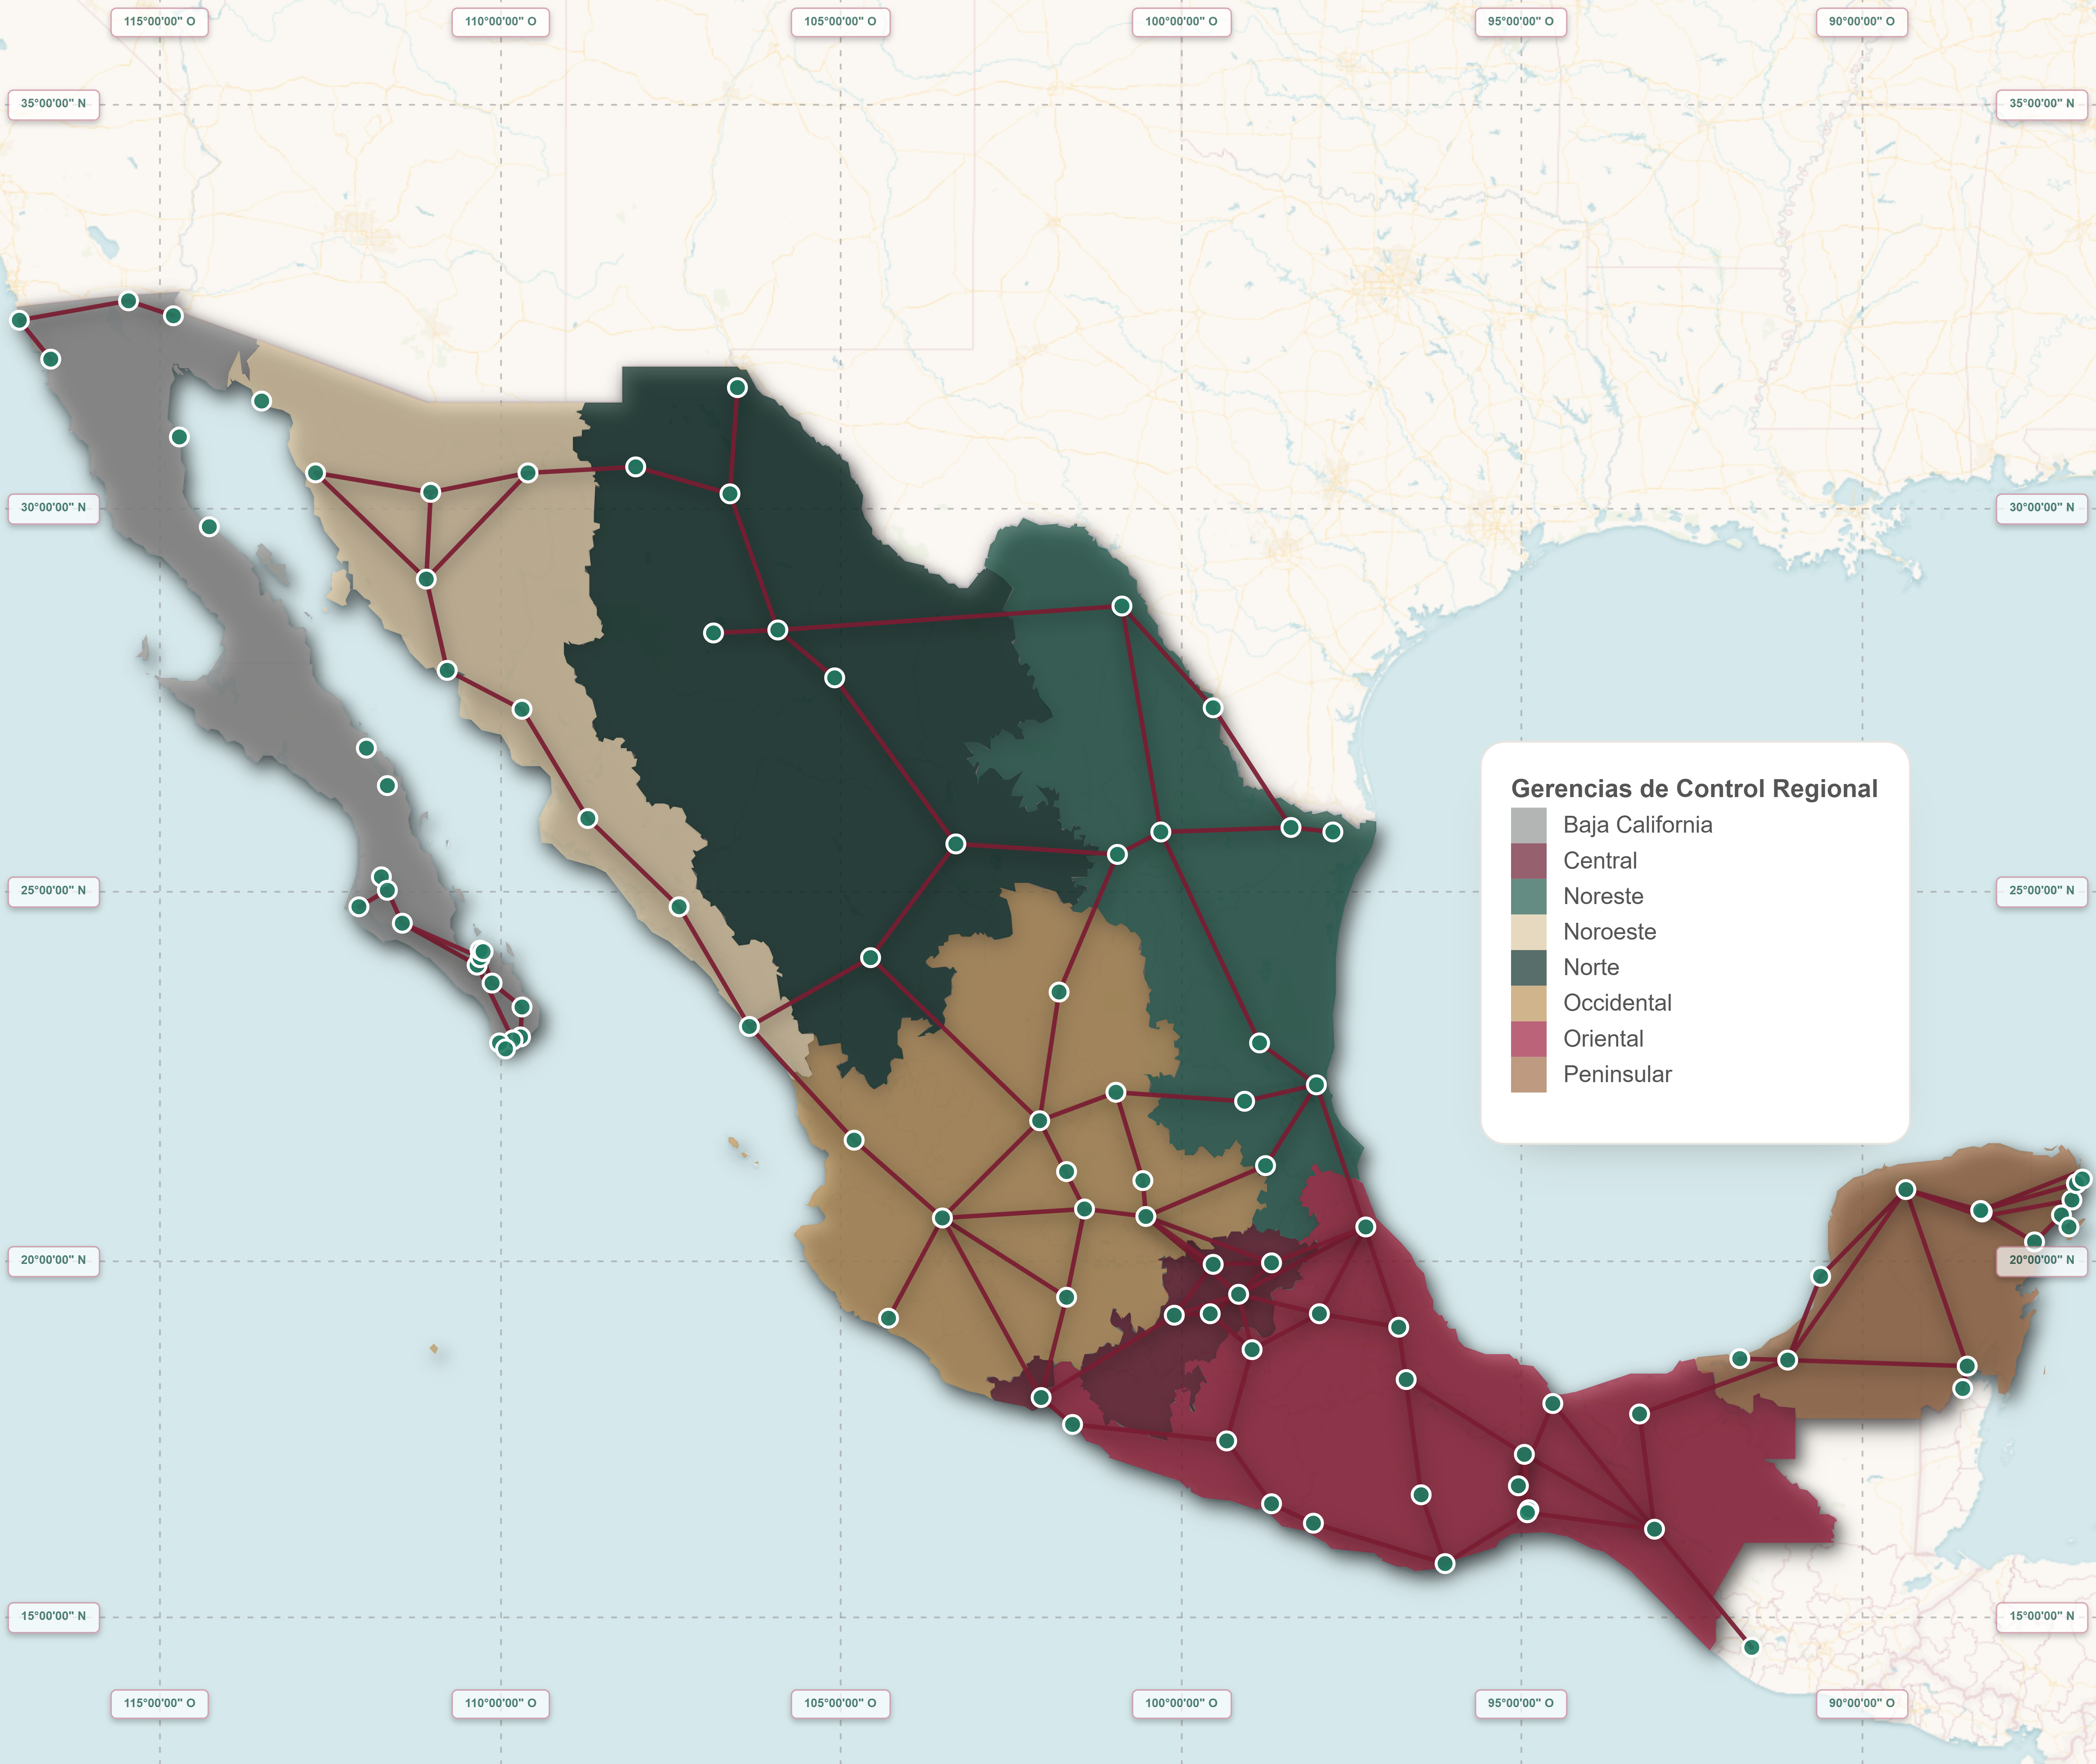
\includegraphics[width=1.0\textwidth]{img/figura_2_1.png}}{Figura 1.1 Principal infraestructura del sector hidrocarburos, 2024}
  \par}
  \raggedright
  \caption{Figura 1.1 Principal infraestructura del sector hidrocarburos, 2024 }
  \label{fig:FIG-1.1-1}
\end{figure}
\vspace{-4pt}
\fuente{Elaboración SENER.\footnote{Nota Fuente}}


probando viñetas:
\begin{itemize}
  \item viñeta 1
  \item viñeta 2
\end{itemize}
sin viñeta:
\begin{itemize}
  \item regresa viñeta
  \item otra viñeta
\end{itemize}
terminan
\begin{itemize}
  \item mas viñetas
\end{itemize}
Texto con \parencite{1} y una nota \footnote{Nota al pie o comentario...}.

Ver [[figura:FIG-1.1-1]] y [[tabla:TBL-1.1-1]].

\begin{equation}
{{km}}^{2}
\end{equation}


\subsubsection{Sub subsección}

Esta es la subsubsección con tabla:

\begin{tabladoradoCorto}
  \caption{Tabñas de Subsección}
  \label{tab:TBL-1.1.1-1}
  \begin{tabularx}{\textwidth}{Vvvv}
    \toprule
    \rowcolor{gobmxDorado} \multicolumn{4}{c}{\encabezadodorado{Concepto}} \\
    \rowcolor{gobmxDorado} \encabezadodorado{a} & \encabezadodorado{b} & \encabezadodorado{c} & \encabezadodorado{d} \\
    \rowcolor{gobmxDorado} \encabezadodorado{uno} & \encabezadodorado{do} & \multicolumn{2}{c}{\encabezadodorado{dos}} \\
    \midrule
    12 & 2 & 3 & 4 \\
    8 & 4 & 45 & 45 \\
    65 & 65 & 654 & 45 \\
    564 & 654 & 56 & 56 \\
    \bottomrule
  \end{tabularx}
\end{tabladoradoCorto}
\vspace{-4pt}
\fuente{Subseccion tabla sencialla 3 fileas de encabezado}



\paragraph{Parrafo}

Este es un parrarfo para el cuarto nivel de jerarquías con tabla larga:

\begin{tablaespecial}
  \captionHorizontal{Tabñas de Subsección larga}
  \label{tab:TBL-1.1.1.1-1}
\begin{tabladoradoLargo}
  \setlength{\SENERLongTableFirstColWidth}{0.34\textwidth}
  \begin{xltabular}{\linewidth}{QZZZZZZZZZZZZZ}
    \toprule
    \rowcolor{gobmxDorado} \encabezadodorado{Cadena} & \encabezadodorado{\SENERVHeader{Carbón mineral}} & \encabezadodorado{\SENERVHeader{Petróleo crudo}} & \encabezadodorado{\SENERVHeader{Condensados}} & \encabezadodorado{\SENERVHeader{Gas natural}} & \encabezadodorado{\SENERVHeader{Energía Nuclear}} & \encabezadodorado{\SENERVHeader{Energia Hidraúlica}} & \encabezadodorado{\SENERVHeader{Geoenergía}} & \encabezadodorado{\SENERVHeader{Energía solar}} & \encabezadodorado{\SENERVHeader{Energía eólica}} & \encabezadodorado{\SENERVHeader{Bagazo de caña}} & \encabezadodorado{\SENERVHeader{Leña}} & \encabezadodorado{\SENERVHeader{Biogás}} & \encabezadodorado{\SENERVHeader{Total energéticos primarios}} \\
    \midrule
    \endfirsthead

    \multicolumn{14}{l}{\small\textit{Continuación...}} \\
    \toprule
    \rowcolor{gobmxDorado} \encabezadodorado{Cadena} & \encabezadodorado{\SENERVHeader{Carbón mineral}} & \encabezadodorado{\SENERVHeader{Petróleo crudo}} & \encabezadodorado{\SENERVHeader{Condensados}} & \encabezadodorado{\SENERVHeader{Gas natural}} & \encabezadodorado{\SENERVHeader{Energía Nuclear}} & \encabezadodorado{\SENERVHeader{Energia Hidraúlica}} & \encabezadodorado{\SENERVHeader{Geoenergía}} & \encabezadodorado{\SENERVHeader{Energía solar}} & \encabezadodorado{\SENERVHeader{Energía eólica}} & \encabezadodorado{\SENERVHeader{Bagazo de caña}} & \encabezadodorado{\SENERVHeader{Leña}} & \encabezadodorado{\SENERVHeader{Biogás}} & \encabezadodorado{\SENERVHeader{Total energéticos primarios}} \\
    \midrule
    \endhead

    \midrule
    \multicolumn{14}{r}{\small\textit{Continúa en la siguiente página...}} \\
    \endfoot

    \bottomrule
    \endlastfoot

    Oferta interna bruta & 219.46 & 1,747.67 & 636.74 & 1,648.09 & 129.51 & 262.18 & 91.32 & 252.18 & 220.18 & 94.72 & 129.42 & 3.25 & 5,434.71 \\
    \hspace{1.35em} Oferta total & 219.56 & 3,674.19 & 637.14 & 1,853.93 & 129.51 & 262.18 & 91.32 & 252.18 & 220.18 & 95.77 & 129.42 & 3.25 & 7,566.61 \\
    \hspace{2.7em} Producción & 14.99 & 3,654.00 & 638.00 & 1,868.00 & 129.51 & 262.18 & 91.32 & 252.18 & 220.18 & 95.77 & 129.42 & 3.25 & 7,358.78 \\
    \hspace{2.7em} Importación & 206.15 & 13.20 & 0.00 & 0.00 & 0.00 & 0.00 & 0.00 & 0.00 & 0.00 & 0.00 & 0.00 & 0.00 & 219.35 \\
    \hspace{2.7em} Variación de inventarios & -1.58 & 6.98 & -0.86 & -14.07 & 0.00 & 0.00 & 0.00 & 0.00 & 0.00 & 0.00 & 0.00 & 0.00 & -9.52 \\
    \hspace{1.35em} Exportación & -0.09 & -1,873.00 & 0.00 & 0.00 & 0.00 & 0.00 & 0.00 & 0.00 & 0.00 & 0.00 & 0.00 & 0.00 & -1,873.09 \\
    \hspace{1.35em} Energía no aprovechada & 0.00 & -53.52 & -0.40 & -205.84 & 0.00 & 0.00 & 0.00 & 0.00 & 0.00 & -1.05 & 0.00 & 0.00 & -260.80 \\
    Total transformaciónes & -147.47 & -1,793.27 & -638.37 & -1,052.40 & -129.51 & -262.18 & -91.32 & -205.70 & -220.18 & -61.50 & 0.00 & -3.25 & -4,605.13 \\
    \hspace{1.35em} Coquizadoras y hornos & 0.00 & 0.00 & 0.00 & 0.00 & 0.00 & 0.00 & 0.00 & 0.00 & 0.00 & 0.00 & 0.00 & 0.00 & 0.00 \\
    \hspace{1.35em} Refinerías y despuntadoras & 0.00 & -1,793.27 & -326.21 & 0.00 & 0.00 & 0.00 & 0.00 & 0.00 & 0.00 & 0.00 & 0.00 & 0.00 & -2,119.48 \\
    \hspace{1.35em} Plantas de gas y fraccionadoras & 0.00 & 0.00 & -312.16 & -1,052.40 & 0.00 & 0.00 & 0.00 & 0.00 & 0.00 & 0.00 & 0.00 & 0.00 & -1,364.56 \\
    \hspace{1.35em} Centrales eléctricas & -147.47 & 0.00 & 0.00 & 0.00 & -129.51 & -262.18 & -91.32 & -205.70 & -220.18 & -61.50 & 0.00 & -3.25 & -1,121.09 \\
    \hspace{2.7em} Carboeléctrica & -147.47 & 0.00 & 0.00 & 0.00 & 0.00 & 0.00 & 0.00 & 0.00 & 0.00 & 0.00 & 0.00 & 0.00 & -147.47 \\
    \hspace{2.7em} Termica convencional & 0.00 & 0.00 & 0.00 & 0.00 & 0.00 & 0.00 & 0.00 & 0.00 & 0.00 & -56.67 & 0.00 & -0.42 & -57.08 \\
    \hspace{2.7em} Combustión interna & 0.00 & 0.00 & 0.00 & 0.00 & 0.00 & 0.00 & 0.00 & 0.00 & 0.00 & -4.83 & 0.00 & 0.00 & -4.83 \\
    \hspace{2.7em} Turbogas & 0.00 & 0.00 & 0.00 & 0.00 & 0.00 & 0.00 & 0.00 & 0.00 & 0.00 & 0.00 & 0.00 & -2.83 & -2.83 \\
    \hspace{2.7em} Ciclo combinado & 0.00 & 0.00 & 0.00 & 0.00 & 0.00 & 0.00 & 0.00 & 0.00 & 0.00 & 0.00 & 0.00 & 0.00 & 0.00 \\
    \hspace{2.7em} Nucleoeléctrica & 0.00 & 0.00 & 0.00 & 0.00 & -129.51 & 0.00 & 0.00 & 0.00 & 0.00 & 0.00 & 0.00 & 0.00 & -129.51 \\
    \hspace{2.7em} Cogeneración & 0.00 & 0.00 & 0.00 & 0.00 & 0.00 & 0.00 & 0.00 & 0.00 & 0.00 & 0.00 & 0.00 & 0.00 & 0.00 \\
    \hspace{2.7em} Hidroeléctrica & 0.00 & 0.00 & 0.00 & 0.00 & 0.00 & -262.18 & 0.00 & 0.00 & 0.00 & 0.00 & 0.00 & 0.00 & -262.18 \\
    \hspace{2.7em} Geotérmica & 0.00 & 0.00 & 0.00 & 0.00 & 0.00 & 0.00 & -91.32 & 0.00 & 0.00 & 0.00 & 0.00 & 0.00 & -91.32 \\
    \hspace{2.7em} Eólica & 0.00 & 0.00 & 0.00 & 0.00 & 0.00 & 0.00 & 0.00 & 0.00 & -220.18 & 0.00 & 0.00 & 0.00 & -220.18 \\
    \hspace{2.7em} Solar fotovoltáica & 0.00 & 0.00 & 0.00 & 0.00 & 0.00 & 0.00 & 0.00 & -205.70 & 0.00 & 0.00 & 0.00 & 0.00 & -205.70 \\
  \end{xltabular}
\end{tabladoradoLargo}
  \fuenteHorizontal{Subseccion tabla sencialla 3 fileas de encabezado}

\end{tablaespecial}



\paragraph{Segundo subparrafo}

Este es el segundo texto del cuarto nivel del indice


\clearpage
\section*{Glosario}
\phantomsection
\addcontentsline{toc}{section}{Glosario}

\entradaGlosario{Centros de Transformación}{Instalaciones industriales de transformación de la energía primaria en productos energéticos secundarios con características que permiten su uso o consumo final.
}
\entradaGlosario{Infraestructura energética}{Conjunto integral de instalaciones, sistemas y tecnologías de gran escala que habilitan el desarrollo, operación, control y mantenimiento de los sectores estratégicos de energía. Esta infraestructura abarca los flujos energéticos del país, incluyendo tanto la infraestructura del Sector Eléctrico como la del Sector Hidrocarburos.}
\entradaGlosario{Sistema Eléctrico Nacional}{Es el conjunto de infraestructura que permite suministrar energía eléctrica a los usuarios finales del país, a través de un sistema integrado por la Red Nacional de Transmisión, la Red Nacional de Distribución, las centrales eléctricas, los equipos e instalaciones del CENACE destinados al control operativo del SEN, así como demás elementos que determine la Secretaría.}

\clearpage
\section*{Siglas y Acrónimos}
\phantomsection
\addcontentsline{toc}{section}{Siglas y Acrónimos}

\entradaSigla{ASA}{Aeropuertos y Servicios Auxiliares}
\entradaSigla{BNE}{Balance Nacional de Energía}
\entradaSigla{CFE}{Comisión Federal de Electricidad}
\entradaSigla{CNE}{Comisión Nacional de Energía}
\entradaSigla{CPEUM}{Constitución Política de los Estados Unidos Mexicanos}

\printbibliography


\end{document}
